\usepgfplotslibrary{fillbetween}

\textbf{Глава 1} посвящена анализу методологии измерения электрического дипольного момента (ЭДМ) 
элементарой частицы при помощи накопительного кольца, работающего в режиме ``замороженного спина.'' 

Глава поделена на три раздела. В разделе 1.1 понятие ``замороженный спин'' определено как состояние, при котором
направление спин-вектора частицы зафиксировано относительно её вектора импульса; 
отмечено преимущество работы в режиме ``замороженного спина,'' а также условия его реализации 
в накопительных кольцах различных типов (чисто электростатические, чисто магнитные, комбинированные).

В разделе 1.2 проводится анализ двух магистральных подходов к измерению ЭДМ частицы в накопительном кольце
с замороженным спином, с целью формулирования критериев успешности методики измерений. Методы
делятся на две категории: 
\begin{enumerate*}[(1)]
	\item методы пространственной области, и 
	\item методы частотной области.
\end{enumerate*}
В методах пространственной области, индикатором ненулевого ЭДМ является отклонение вектора поляризации 
изначально полностью продольно-поляризованного пучка от плоскости замкнутой орбиты. В методах частотной
области, показателем отличия ЭДМ от нуля является разница между частотами прецессии спинов частиц пучка в 
экспериментах с противоположным течением времени.

Систематизируются основные проблемы, возникающие при попытке измерить ЭДМ частицы 
в накопительном кольце при любом из существующих подходов:
\begin{enumerate}[(1)]
	\item возмущения спиновой динамики частиц;
	\item спин-декогеренция;
	\item неидеальности оптической структуры ускорителя. (Вызывает фальш-сигнал ЭДМ.)
\end{enumerate}

В подразделе 1.2.5 описывается метод (Frequency Domain Method), разработанный с целью решения 
всех поставленных выше проблем.

Метод основан на утверждении об эквивалентности, с точки зрения спиновой динамики, 
частиц с одинаковым равновесным уровнем энергии -- в независимости от их траекторий. 
Для доказательства этого утверждения, в подразделе 1.2.6 вводится понятие \emph{эффективного Лоренц-фактора}, 
позволяющего учесть влияние удлинения орбиты частицы (за счёт бетатронного движения и дисперсии)
на её частоту прецессии спина.

В резделе 1.3 представлены три варианта магнитооптической структуры кольца 
для измерения ЭДМ дейтрона предлагаемым методом: одна структура (FS) 
реализует классическое определение ``замороженности'' спина (т.е. горизонтальные проекции 
спин-вектора и вектора импульса частицы сонаправлены в каждый момент времени),
две другие  реализуют состояние ``квази-замороженного спина'' (QFS). 

\begin{figure}[H]\centering
	\includegraphics[width=.95\linewidth]{images/chapter2/BNL_lattice}
	\caption{Магнитооптическая структура кольца с ``замороженным спином''\label{fig:lattices:FS}}
\end{figure}
\begin{figure}[H]\centering
	\includegraphics[width=.95\linewidth, trim=0 3 0 0, clip]{images/chapter2/6_3_lattice}
	\caption{Магнитооптическая структура кольца с ``квази-замороженным спином,'' 
		с пространственно-разделёнными E- и B-полями\label{fig:lattices:6_3}}
\end{figure}
\begin{figure}[H]\centering
	\includegraphics[width=.95\linewidth]{images/chapter2/E+B_lattice}
\caption{Магнитооптическая структура накопительного кольца с ``квази-замороженным спином,'' 
	с пространственно-совмещёнными E- и B-полями\label{fig:lattices:E+B}}
\end{figure}

Необходимость разработки QFS-структур обусловлена тем, 
что даже в FS-структуре (Рисунок~\ref{fig:lattices:FS}), условие замороженности спина, 
хотя и обеспечивает \emph{максимальную} амплитуду ЭДМ-сигнала, 
выполняется строго только для референсной частицы. 
При этом, FS-структура требует использование цилиндрических спин-ротаторов 
с совмещёнными электрическим и магнитным полями. 

Преимущество кольца QFS-типа сосоит в относительной простоте исполнения: 
в предложенных вариантах, используются либо
\begin{enumerate}[(\bfseries i\normalfont)]
	\item цилиндрические электростатические дефлекторы и магнитные диполи раздельно
	 (Рисунок~\ref{fig:lattices:6_3}), либо
	\item прямые фильтры Вина (Рисунок~\ref{fig:lattices:E+B}).	
\end{enumerate}
Простота исполнения, в свою очередь, позволяет использовать QFS структуру в неспециализированном под
измерения ЭДМ накопительном кольце.

\textbf{Глава 2} посвящена анализу проблем измерения ЭДМ частицы 
в накопительном кольце с замороженным спином, и поиску их решений. 

Рассматриваются следующие проблемы:

\textbf{Возмущения спиновой динамики частицы} вызванные её бетатронными колебаниями, и их эффект на ЭДМ-статистику частотного метода измерений (раздел 2.1).

Суть проблемы в следующем: частота прецессии спина, на основании которой делаются выводы о величине ЭДМ в 
методах частотной области, вычисляется посредством фитирования гармонической функции 
${f(t) = a\cdot\sin(\w\cdot t + \phi)}$ с \emph{постоянными} параметрами $(a,\w,\phi)$. При этом, для частиц, вовлечённых
в бетатронное движение, решение уравнения спин-динамики (уравнение Томаса-Баргманна-Мишеля-Телегди)
для вертикальной компоненты спин-вектора:
\begin{equation}\label{eq:sy_analytic}
s_y = \sqrt{\bkt{\bar n_y\bar n_z}^2 + \bar n_x^2} \cdot \sin\bkt{2\pi\cdot\nu_s\cdot \frac{t}{T} + \phi},
\end{equation}
где $\nbar$ -- ось стабильного спина частицы -- \emph{меняет своё направление} во время бетатронного движения.~\cite[стр.~11]{Shatunov} Несоответствие между фитируемым сигналом и моделью влечёт за собой
систематическую ошибку в оценке параметров модели. На сколько вариация в амплитуды колебаний вертикальной
компоненты поляризации влияет на систематическую ошибку оценки частоты колебаний -- 
и был интересовавший нас вопрос.

В ходе численного моделирования, мы получили данные, представленные на Рисунке~\ref{fig:sd}. 
\begin{figure}[H]\centering
	\subbottom[Компонент $\bar n$\label{fig:sd:nbar}]{%
		\includegraphics[height=.33\paperheight]{images/smp_sim/NBAR_variation_sd_vs_SW}}
\end{figure}
\begin{figure}[H]\centering
	\contsubbottom[Сравнительных невязок.
	Верхняя панель: невязка $\epsilon_1$; нижняя панель: невязка $\epsilon_2$\label{fig:sd:res}]{%
		\includegraphics[height=.33\paperheight]{images/smp_sim/residual_SD_vs_SW(both)}}
	\caption{Стандартные отклонения в зависимости от относительной частоты МДМ спин-прецессии\label{fig:sd}}
\end{figure}

Здесь, сравнительные невязки ${\epsilon_1 = s_y^{gen} - s_y^{idl}}$, ${\epsilon_2 = S_y^{trk} - s_y^{idl}}$,
где временн\'{а}я серия $s_y^{trk}(t)$ получена посредством трекинга частиц 
в коде COSY INFINITY~\cite{COSYINF:Website}; $s_y^{gen}(t)$ получена из уравнения~\eqref{eq:sy_analytic}
при подстановке значений $\nu_s(t)$ и $\nbar(t)$, а $s_y^{idl}(t)$ -- при подстановке ${\nu_s=\avg{\nu_s(t)}}$ и 
${\nbar = \avg{\nbar(t)}}$.

%Исходя из наблюдаемого на Рисунке~\ref{fig:sd} поведения стандартных отклонений невязок 
%$\epsilon_1$ и $\epsilon_2$, был сделан вывод о пренебрежимости эффектом прецессии 
%осей стабильного спина частиц пучка.

Основные выводы, сделанные на основе анализа данных симуляции, таковы:
\begin{enumerate}
	\item Осцилляции амплитуды сигнала очень малы. Они происходят на уровне не более $10^{-4}$ (при
	${\alpha\sim N(0, 3\cdot 10^{-2})}$ градусов), тогда как ожидаемая неточность измерений поляризации находится
	на уровне процентов. Это значит, что суперпозиция систематической ошибки и случайной ошибки измерения
	не будет проявлять статистически-значимую систематичность.
	\item Коэффициент корреляции между оценками амплитуды и частоты не значителен. Колебания амплитуды
	влияют на оценку $\hat a$ в первую очередь; их эффект на оценку $\hat\w$ опосредован, и описывается
	коэффициентом корреляции. Поскольку он меньше 10\%, даже если колебания окажутся достаточными, чтобы повлиять
	на оценку амплитуды, их эффект на оценку частоты будет уменьшен по крайней мере в 10 раз.
	\item Этот систематический эффект контролируется. И этот фактор является основным достоинством методологий
	частотной области. Вводя в систему внешнее магнитное поле (SW на Рисунке~\ref{fig:sd}), 
	колебания $\bar n$ могут быть 
	непрерывно минимизированы  до необходимого уровня, без каких-либо модификаций паттерна эксперимента.
\end{enumerate}

\textbf{Декогеренция спинов} частиц продольно-поляризованного пучка 
при работе в режиме замороженного спина (раздел 2.2).

Проблема спин-декогеренции пучка вызвана различием частот прецессии спинов частиц пучка, 
что в свою очередь связано с разницей равновесных уровней энергии частиц. 

Для решения проблемы спин-декогеренции применяют~\cite{COSY:SCT:IPAC15, COSY:SCT:1000sec} 
нелинейные элементы (секступоли), влияющие одновременно на длины орбит бетатрон-осциллирующих частиц,  
и на коэффициент сжатия орбиты ${\alpha = \alpha_0 + \alpha_1\delta}$ (где ${\delta=\Delta p/p_0}$).

В подразделе 2.2.4 описаны результаты численного моделирования секступольного подавления спин-декогеренции 
в идеально отъюстированном (т.е. отсутствует МДМ спин-прецессия вокруг радиальной оси) накопительном кольце 
FS-типа (Рисунок~\ref{fig:lattices:FS}). В результате симуляции были получены данные, представленные на Рисунке~\ref{fig:decoh:perfect}. Как следует из рисунка, при включении секступольных полей теряется зависимость
нормированной частоты прецессии спина частицы (спин-тюна) от её координаты в поперечной к оптической оси
 плоскости ($x$--$y$) и от её энергии $\delta = \Delta K/K_0$ 
 (где $K$ -- кинетическая энергия частицы, индекс 0 обозначает референсную частицу).

\begin{figure}[H]
	\centering
	\subbottom[В горизонтальном направлении]{%
		\includegraphics[height=.3\paperheight]{images/decoh_sim/spin_tune_decoh_x_offset}}
\end{figure}
\begin{figure}[H]\centering
	\contsubbottom[В вертикальном направлении]{%
		\includegraphics[height=.3\paperheight]{images/decoh_sim/spin_tune_decoh_y_offset}}
%\end{figure}
%\begin{figure}[H]\centering
	\subbottom[По энергии]{%
		\includegraphics[height=.3\paperheight]{images/decoh_sim/spin_tune_decoh_d_offset_1}}
	\legend{Цветом выделены зависимости при нулевом (чёрный) и оптимизированном (красный) значениях градиента секступоля}
	\caption{Зависимость спин-тюна частицы от её смещения от референсной частицы\label{fig:decoh:perfect}}
\end{figure}

Существует предположение~\cite[стр.~5]{Koop:SpinWheel2015}, что появление радиальной компоненты МДМ спин-прецесии подавляет спин-декогеренцию. В подразделе 2.2.5 показано, что появление 
радиальной компоненты МДМ спин-прецессии само по себе не подавляет спин-декогеренцию, 
а только меняет плоскость, в которой она происходит (из горизонтальной в вертикальную). 

В подразделе 2.2.6 описаны результаты численного моделирования секступольного метода 
подавления спин-декогеренции в неидеальном ускорителе; на основе этой симуляции был проанализирован
эффект секступольных подей на спин-тюн частицы, а также и на направление её оси стабильного спина. 
По результатам анализа был сделан важный вывод: секступольные поля выравнивают не только спин-тюны
частиц банча, но и направления их осей стабильного спина (см. Рисунок~\ref{decoh:fig:nbar_vs_ST}).

%\begin{figure}[H]\centering
%	\subbottom[С выключенными секступолями]{%
%		\includegraphics[height=.33\paperheight]{images/decoh_sim/NX_VS_YB_IMPERFECT_UNOPT}}
%\end{figure}
%\begin{figure}[H]\centering
%	\contsubbottom[С включенными секступолями]{%
%		\includegraphics[height=.33\paperheight]{images/decoh_sim/NX_VS_YB_IMPERFECT_OPTIM}}
%	\caption{Радиальные компоненты осей прецессии спинов частиц на их траекториях в неидеальной FS-структуре\label{decoh:fig:NX_on_traj}}
%\end{figure}
%
%\begin{figure}[H]\centering
%	\subbottom[С выключенными секступолями]{%
%		\includegraphics[height=.33\paperheight]{images/decoh_sim/NY_VS_YB_IMPERFECT_UNOPT}}
%\end{figure}
%\begin{figure}[H]\centering
%	\contsubbottom[С включенными секступолями]{%
%		\includegraphics[height=.33\paperheight]{images/decoh_sim/NY_VS_YB_IMPERFECT_OPTIM}}
%	\caption{Вертикальные компоненты осей прецессии спинов частиц на их траекториях в неидеальной FS-структуре\label{decoh:fig:NY_on_traj}}
%\end{figure}
%
%\begin{figure}[H]\centering
%	\subbottom[С выключенными секступолями]{%
%		\includegraphics[height=.33\paperheight]{images/decoh_sim/NZ_VS_YB_IMPERFECT_UNOPT}}
%\end{figure}
%\begin{figure}[H]\centering
%	\contsubbottom[С включенными секступолями]{%
%		\includegraphics[height=.33\paperheight]{images/decoh_sim/NZ_VS_YB_IMPERFECT_OPTIM}}
%	\caption{Продольные компоненты осей прецессии спинов частиц на их траекториях в неидеальной FS-структуре\label{decoh:fig:NZ_on_traj}}
%\end{figure}

\begin{figure}[H]\centering
	\includegraphics[height=.35\paperheight]{images/decoh_sim/mean_n_bar_vs_spin_tune}
	\caption{Средние уровни поперечных компонент осей стабильного спина частиц, в зависимости от уровня их спин-тюна.\label{decoh:fig:nbar_vs_ST}}
\end{figure}

В подразделе 2.2.7 анализируется механизм подавления спин-декогеренции секступольными полями. 
Как было отмечено ранее, секступольное поле влияет на декогеренцию двумя путями: 
модифицируя коэффициент сжатия орбиты, и длину орбиты частицы.
По этой причине, для анализа использовались два теста. В первом, все частицы пучка (D-банча) 
инжектируются на замкнутую орбиту, и различаются только начальным уровнем кинетической энергии. 
Поскольку при варьировании поля секступоля длины орбит частиц не меняются, первый тест 
показывает эффект варьирования только коэффициента сжатия орбиты на зависимость спин-тюна частицы
от её равновесного уровня энергии. Результаты представлены на Рисунке~\ref{fig:decoh_anal:D-bunch}.
\begin{figure}[H]\centering
	\subbottom[Фазовые эллипсы при различных значениях градиента секступоля]{%
		\includegraphics[height=.26\paperheight]{images/decoh_sim/propdef/long_phase_space_for_sext_settings_D}
	}
%\end{figure}
%\begin{figure}[H]\centering
	\subbottom[Зависимость среднего уровня спин-тюна частицы от её равновесного уровня энергии для различных значений градиента секступоля\label{fig:decoh_anal:D-bunch:sign}]{%
		\includegraphics[height=.26\paperheight]{images/decoh_sim/propdef/stune_vs_dkok_SS_D}
	}
\caption{Фазовые портреты и функциональная зависимость спин-тюна частицы от её равновесного уровня энергии для D-банча\label{fig:decoh_anal:D-bunch}}
\end{figure}

Мы отмечаем две вещи: 
\begin{enumerate*}[(1)]
	\item скученность центров фазовых эллипсов/точек на графике~\ref{fig:decoh_anal:D-bunch:sign} не меняется
	при вариации градиента секступоля;
	\item функциональная зависимость на графике~\ref{fig:decoh_anal:D-bunch:sign} меняется
	при вариации градиента секступоля.
\end{enumerate*}
%
Скученность центров фазовых эллипсов ассоциируется с дисперсией длин орбит частиц; 
функциональная зависимость ${\nu_s = f(\avg{\Delta K/K}; \alpha_1)}$ -- с коэффициентом сжатия орбиты.

Во втором тесте, частицы (Y-банч) инжектировались на одной и той же энергии, 
но с различным начальным вертикальным смещением от замкнутой орбиты, 
т.е. совершали бетатронные колебания в вертикальной плоскости (в добавок к синхротронным колебаниям).
Результаты теста представлены на Рисунке~\ref{fig:decoh_anal:Y-bunch}.

\begin{figure}[H]\centering
	\subbottom[Фазовые эллипсы при различных значениях градиента секступоля\label{fig:decoh_anal:Y-bunch:ps}]{%
		\includegraphics[height=.26\paperheight]{images/decoh_sim/propdef/long_phase_space_for_sext_settings_Y}
	}
%\end{figure}
%\begin{figure}[H]\centering
	\subbottom[Фазовые портреты и функциональная зависимость спин-тюна частицы от её равновесного уровня энергии для Y-банча]{%
		\includegraphics[height=.26\paperheight]{images/decoh_sim/propdef/stune_vs_dkok_SS_Y}
	}
	\caption{Фазовые портреты и функциональная зависимость спин-тюна частицы от её равновесного уровня энергии для Y-банча\label{fig:decoh_anal:Y-bunch}}
\end{figure}

В данном случае отметим:
\begin{enumerate*}[(1)]
	\item изменение скученности центров фазовых эллипсов, т.е. влияние вариации градиента секступоля 
	на длины орбит частиц;
	\item изменение функциональной зависимости ${\nu_s = f(\avg{\Delta K/K}; \alpha_1)}$;
	\item оптимальное значение градиента секступоля (средняя панель на Рисунке~\ref{fig:decoh_anal:Y-bunch:ps}) 
	не соответствует минимальному размеру фазовых эллипсов.
\end{enumerate*}

Свойства \textbf{МДМ компоненты частоты спин-прецессии вокруг радиальной оси} $\W_x^{MDM}$, вызванной 
неидеальностями оптической структуры ускорителя, и составляющей основную 
систематическую ошибку измерений ЭДМ в накопительном кольце (любым из методов), анализируются в разделе 2.3.

В подразделе 2.3.1 подтверждаются следующие свойства $\W_x^{MDM}$ (см. Рисунок~\ref{fig:syst:linearity}):
\begin{enumerate}[(1)]
	\item зависимость $\W_x^{MDM}$ \emph{только} от среднего угла наклона спин-ротаторов $\avg{\Theta_{tilt}}$, 
	но \emph{не} от конкретной последовательности наклонов элементов $\{\Theta_{tilt}^{(i)}\}_{i\in J}$;
	\item зависимость $\W_x^{MDM}(\avg{\Theta_{tilt}}) = L(\avg{\Theta_{tilt}})$ носит линейный характер.
\end{enumerate}

\begin{figure}[H]\centering
	\includegraphics[height=.35\paperheight]{images/fake_signal_sim/linearity_test_shifting_gauss_freq}
	\caption{Зависимость компонент частоты МДМ спин-прецессии $\vec\W^{MDM}$ референсной частицы 
		в неидеальной FS-структуре~\ref{fig:lattices:FS} 
		со случайно-распределёнными ошибками установки спин-ротаторов 
		от их среднего угла наклона $\avg{\Theta_{tilt}}$\label{fig:syst:linearity}}
\end{figure}

В подразделе 2.3.2 величина $\W_x^{MDM}$ сравнивается для двух противоположных направлений движения пучка:
по (CW) и против (CCW) часовой стрелки. Результаты симуляции представлены на Рисунке~\ref{fig:syst:asym}.

\begin{figure}[H]\centering
	\includegraphics[height=.35\paperheight]{images/fake_signal_sim/linearity_test_shifting_gauss_rel_diff}	
	\caption{Относительная разница между радиальными компонентами оси стабильного спина и угловой скоростью поворота спина, посчитанная относительно значения для CW-циркулирующего пучка\label{fig:syst:asym}}
\end{figure}

По результатам симуляции сделан вывод о том, что при движении пучка в любом из направлений 
ось стабильного спина $\nbar$ наклонена одинаково; при этом существует \emph{различие} 
между спин-тюнами CW и CCW пучков, но на уровне не более десятых долей процента, 
которое тем сильнее, чем меньше модуль $\W_x^{MDM}$. 
Эта \emph{разница}  свидетельствует об асимметричности ускорительной структуры 
относительно обращения направления движения, с точки зрения спиновой динамики, 
и может объясняться различием референсных орбит CW и CCW пучков. 

Проблема \textbf{смены полярности ведущего поля ускорителя} рассмотрена в разделе 2.4 . 
Эта процедура необходима для смены направления движения дейтронного пучка, 
т.е. для сокращения МДМ компоненты совокупной частоты прецессии, измеряемой в методах частотной области. 

Необходимо отметить, что целью смены полярности ведущего поля является 
точное воспроизведение радиальной компоненты частоты МДМ прецессии $\W_x^{MDM}$, 
индуцированной полями неидеальности оптической структуры ускорителя. 
Этот момент часто упускается из виду: простое воспроизведение величины \emph{магнитного поля} 
не достаточно, поскольку точка инжекции центроида пучка, а значит его длина орбиты --- 
и, соответственно, спин-тюн, --- подвержена вариации. Не говоря о возможной асимметричности 
оптической структуры кольца, с точки зрения спиновой динамики, относительно 
обращения направления движения пучка. Таким образом, необходимо восстанавливать не величину поля, 
а эффективный Лоренц-фактор центроида.

Для калибровки эффективного Лоренц-фактора, в \emph{FD}-методе измеряется вертикальная компонента
ЭДМ+МДМ частоты спин-прецессии $\W_y$; пучок при этом выводится из состояния ``замороженного спина.'' 

В результате симуляции, были получены результаты, представленные на Рисунке~\ref{fig:calib}.

Можно видеть, что при уменьшении разницы ${\Delta\W_y^{MDM} < 10^{-7}}$~рад/сек 
(точность определения частоты, достигаемая при фитировании данных с одного цикла), 
разница ${\Delta \W_x^{MDM} < 10^{-8}}$~рад/сек (т.е. на порядок меньше статистической погрешности). 
Это говорит о принципиальной возможности использования частоты прецессии спина в горизонтальной плоскости 
для калибровки частоты прецессии в вертикальной плоскости.

\begin{figure}[H]\centering
	\subbottom[Результаты симуляции для случая декогеренции, вызванной
	бетатронным движением в горизонтальной плоскости]{%
		\includegraphics[height=.33\paperheight]{images/GFF/GFF_omegas_range_X}}
\end{figure}
\begin{figure}[H]\centering
	\contsubbottom[Результаты симуляции для случая декогеренции, вызванной
	бетатронным движением в вертикальной плоскости]{%
		\includegraphics[height=.33\paperheight]{images/GFF/GFF_omegas_range_Y}}
%\end{figure}
%\begin{figure}[H]\centering
	\contsubbottom[Результаты симуляции для случая декогеренции, вызванной
	синхротронным движением]{%
		\includegraphics[height=.33\paperheight]{images/GFF/GFF_omegas_range_D}}
	\caption{Разница между радиальными компонентами частоты прецессии CW и CCW пучков
		в зависимости от разницы вертикальных компонент (калибровочный график)\label{fig:calib}}
\end{figure}

Отдельно, в разделе 2.5, рассматривается вопрос интерпретации введённого в подразделе 1.2.6 понятия 
\textbf{эффективного Лоренц-фактора} ($\gamma_{eff}$). 

Больш\'{а}я часть методологии, исследованию которой посвящена настоящая работа, основана на утверждении: 
частицы с одинаковым значением эффективного Лоренц-фактора имеют одинаковый спин-тюн, 
то есть эквивалентны с точки зрения спиновой динамики.

Раздел поделён на два подраздела. В подразделе 2.5.1 эффективный Лоренц фактор интерпретируется как 
математическое ожидание кинетической энергии частицы. Такая интерпретация предполагалась при введении
этого понятия, однако она не подтвердилась. В подразделе 2.5.2 был принят более абстрактный подход: 
был поставлен вопрос о возможности сведения функции многих переменных $\nu_s(x,a,y,b,\ell,\delta)$ 
к функции одной переменной $\nu_s(\gamma_{eff})$. Возможность подтверждена, эффективный Лоренц-фактор
интерпретируется как мера продольного эмиттанса пучка.

\textbf{Глава 3} посвящена статистическому моделированию эксперимента, 
и оценке его возможной статистической точности. Исследуется возможность повышения эффективности
поляриметрии путём использования частотно-модулированной схемы выборки. Модулированная схема 
состоит в том, чтобы измерять поляризацию пучка в момент максимальной скорости её изменения 
(см. Рисунок~\ref{fig:modulated_sampling}).

\begin{figure}[H]\centering
	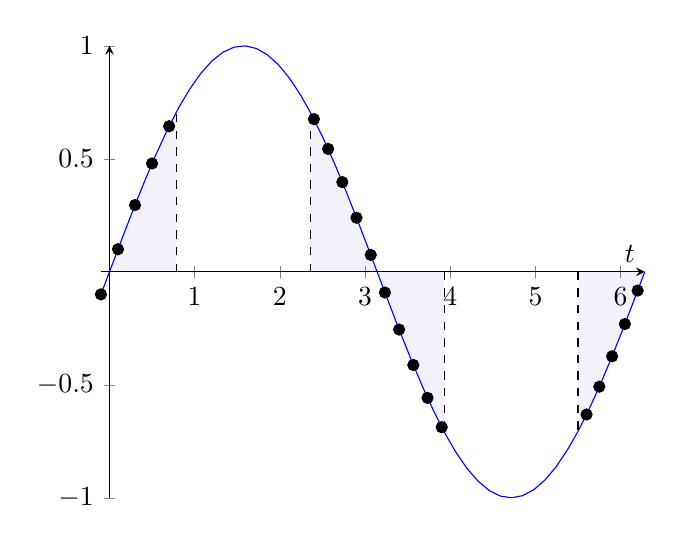
\begin{tikzpicture}
	\begin{axis}[axis lines=center, xlabel=$t$, domain=-.5:2*pi, legend pos=outer north east, width=.7\textwidth,
	scatter/use mapped color={draw=black, fill=black}
	]
	\addplot[color=blue, name path=signal, domain=-.1:2*pi,samples=50] {sin(deg(x))};
	\draw[dashed] (axis cs:.785,0) -- (axis cs:.785,{sin(deg(.785))});
	\draw[dashed] (axis cs:2.36,0) -- (axis cs:2.36,{sin(deg(2.36))});
	\draw[dashed] (axis cs:3.93,0) -- (axis cs:3.93,{sin(deg(3.93))});
	\draw[dashed] (axis cs:5.5,0) -- (axis cs:5.5,{sin(deg(5.5))});
	\path[name path=axis] (axis cs:0,0) -- (axis cs:2*pi,0);
	\addplot[fill=blue, opacity=.05] fill between [of=signal and axis, soft clip={domain=0:.785}];
	\addplot[fill=blue, opacity=.05] fill between [of=signal and axis, soft clip={domain=2.36:3.93}];
	\addplot[fill=blue, opacity=.05] fill between [of=signal and axis, soft clip={domain=5.5:2*pi}];
	\addplot [scatter, only marks, domain=-.1:.7, samples=5] {sin(deg(x))};
	\addplot [scatter, only marks, domain=2.4:3.9, samples=10, mark=*] {sin(deg(x))};
	\addplot [scatter, only marks, domain=5.6:6.2, samples=5, mark=*] {sin(deg(x))};
	\end{axis}     
	\end{tikzpicture}
	\caption{Частотно-модулированная выборка: измерения делаются только в максимально информативных точках,
		находящихся в окрестностях узлов сигнала\label{fig:modulated_sampling}}
\end{figure}

Мы приходим к выводу о нецелесообразности использования модулированной схемы выборки. Она даёт только
малый выигрыш (40\%) по сравнению с немодулированной схемой, \emph{даже если} не учитывать вариацию 
анализирующей способности детектора. Учитывая, что максимальная скорость изменения соответствует
окрестности продольной ориентации вектора поляризации пучка, в которой анализирующая способность 
детектора минимальна, полезность модулированной схемы ещё меньше.

Также важно отметить отсутствие прямой зависимости между частотой $\omega$ измеряемого сигнала, 
и стандартным отклонением оценки частоты $\sigma_{\hat\omega}$. То есть, нет принципиальной разницы
измеряется ли частота в 1 или 100~рад/сек. Это обстоятельство важно для методов детектирования ЭДМ, 
основанных на измерении частоты прецессии спина: благодаря ему, строго говоря, 
отсутствует необходимость подавлять МДМ-прецессию, связанную с неидеальностями 
оптической структуры ускорителя.

Также, была оценена эффективная длительность измерительного цикла, 
исходя из времени жизни поляризации пучка  $\tau_d$ (опеределяемого как период времени, 
за который полярищация пучка уменьшается в $e$ раз). Очевидно, что когда пучок полностью деполяризуется, 
мы не сможем получать информацию о скорости вращения его поляризации; т.е. 
существует принципиальное ограничение на полное количество информации (обозначим её $\mathrm{FI_{tot}}$) 
о частоте прецессии спина, которое можно получить из одной инжекции.
В таблице~\ref{tbl:FItot} отражено количество выбранной (относительно $\mathrm{FI_{tot}}$) информации 
о частоте прецессии спина как функция длительности цикла, а также соответствующее отношение
сигнал/шум. Исходя из данных таблицы, полезная длительность измерительного цикла 
ограничена тремя постоянными времени деполяризации.

Результаты численного моделирования~\cite{Aksentev:Stats} показывают 
возможность достичь точности оценки частоты прецессии спина 
на уровне ${8\cdot 10^{-7}}$ рад/сек за один измерительный цикл, при постоянной времени деполяризации 
1 000~сек, частоте измерения поляризации 375~Гц, и начальной ошибке измерения поляризации 3\%. 
При 70\%  годовой временной загрузке ускорителя, это позволяет выйти на уровень 
${5\cdot 10^{-9}}$~рад/сек стандартного отклонения среднего значения оценки частоты. 
Такая точность достаточна для получения оценки ЭДМ на уровне $10^{-29}~e\cdot$см.

\begin{table}[H]
	\caption{Количество выбранной информации (в долях от потенциального максимума), 
		в зависимости от длительности измерительного цикла, 
		и соответствующее отношение сигнал/шум.\label{tbl:FItot}}
	\centering
	\begin{tabular}{rrr}
		\toprule
		Инфо. (\%$\mathrm{FI_{tot}}$) & Длительность ($\times\tau_d$) & Сигнал/шум  \\
		\midrule
		95            & 3.0                     & 0.4         \\
		90            & 2.3                     & 1.1         \\
		70            & 1.2                     & 5.5         \\
		50            & 0.7                     & 11.7        \\
		\bottomrule
	\end{tabular}
\end{table}

В \textbf{Главе 4} описаны наиболее значимые (для данной работы) технологии, 
разработанные в рамках исследований, проводимых на синхротроне COSY (Рисунок~\ref{fig:COSY_Ring}), 
а также описаны результаты процедуры оптимизации времени когерентности спина (spin coherence time, SCT) 
при помощи семейств секступолей, установленных на COSY
(параметры COSY  представлены в Таблице~\ref{tbl:COSY-studies}).

\begin{figure}[H]\centering
	\includegraphics[width=\linewidth]{images/chapter4/COSY-sextupoles}
	\caption{Кольцо COSY с отмеченными положениями секступолей для контроля времени когерентности спина. (Рисунок взят из~\cite{Guidoboni:STORI14})\label{fig:COSY_Ring}}
\end{figure}


\begin{table}[H]\centering
	\caption{Рабочие параметры COSY, использованные в проводимых исследованиях\label{tbl:COSY-studies}}
	\begin{tabular}{lll}
		\toprule
		Параметр & Величина & Размерность \\
		\midrule
		Длина окружности COSY& 183 & м\\
		Импульс дейтрона & 970 & МэВ/с \\
		$\beta$ / $\gamma$ & 0.459 / 1.126 & \\
		Аномальный магнитный момент G& -0.143& \\
		Частота оборота пучка $f_{\mathrm{rev}}$& 752543& Гц\\
		Длительность измерительного цикла& 100--1500& сек\\
		Число частиц в пучке & $\approx 10^9$& \\
		\bottomrule
	\end{tabular}
\end{table}

Описанные технологии:
\begin{enumerate}[(1)]
	\item высокоточное измерение спин-тюна (с точностью до $10^{-10}$ в измерительном цикле 100~секунд);
	\item юстировка квадруполей при помощи пучка (Beam Based Alignment~\cite{Wagner:BBA2018});
	\item оптимизация времени когерентности спина~\cite{COSY:SCT:IPAC15, Guidoboni:STORI14}.
\end{enumerate} 

Отдельно стоит отметить наблюдение явления изменения SCT (см. Рисунок~\ref{fig:April2019:Polarization}) 
при длительном измерении поляризации деструктивными методами, связаного с переходом 
от внешней (оболочки) к внутренней (ядру) частям пучка. 
Наблюдение этого явления косвенно подтверждает теорию спин-декогеренции, изложенную в данной работе.

\begin{figure}[H]\centering
	\includegraphics[height=.3\paperheight]{images/chapter4/SCT-April-2019/11th_20-20}
\caption{Измерения горизонтальной поляризации во время оптимизации времени когерентности спина при подготовке к эксперименту по поиску аксионов в апреле 2019 года\label{fig:April2019:Polarization}}
\end{figure}
